\section{Introduction}
Matched-field processing (MFP) is a common technique for source localization in an acoustic
wave-guide\cite{bucker1976use,baggeroer1988matched,baggeroer1993overview}.
MFP localization matches measured acoustic pressure field data on an array of sensors with a replica field computed by a numerical propagation model for an assumed source range and depth. The processor output is maximum at the true source range and depth. However, MFP requires a pretty good knowledge of environment, which means significant errors in the environment model can be introduced into the
depth and range localization predictions\cite{tolstoy1989sensitivity,del1988effects}.

Machine learning methods do not require a good a prior information and can implement a required calculation through learning from examples. A well designed structure can learn a generic model that works in different kinds of scenarios. This is meaningful for us to improve the robustness of conventional methods by introducing machine learning methods into underwater acoustics.
Machine learning  has obtained success in many areas, such as speech recognition, natural language processing and image processing. There are also applications in underwater acoustics.
Previous works have used artificial neural networks to classify whale sounds\cite{thode2012automated}, locate targets area\cite{steinberg1991neural} and discriminate depth\cite{ozard1991artificial}.
A notable recent example using machine learning methods in underwater acoustic is the application of nonlinear classification to source localization\cite{niu2017source}. There is no discussion on how using machine learning to help solve the mismatch problem in underwater acoustics.

In this paper, the source localization problem is viewed within a machine learning
framework. As the sound-speed profile (SSP) in the water layer is the most important parameter needed to be known accurately\cite{feuillade1989environmental}, we primary focus on the SSP
mismatch problem.
Two different degrees of error (a large one and a slight one) in the knowledge of the sound-speed profile are chose to train and test the model.
The large one has significant change in shape, while the slight one just has small shift (within 0.5m/s at the same depth) in sound speed.
Effects of such errors on positioning performance for various methods, including Bartlett matched-field processing, matched-covariance estimation (MCE) and feed-forward neural networks based method (FNN), are compared.
Treat different SSPs as different application scenes, and then a generic model is learned by data-model mixed training, the trained model is tested on
different SSPs.
In Niu's work\cite{niu2017source}, he used a dense neural networks to train his model, the model performs well on the data of Noise09 experiment, which verified that FNN can achieve a good prediction performance when source localization is solved as a classification problem. However, as he said, the FNN classifier will be over-fitting and predict poorly when the SNR of training data is low. In order to overcome this problem,
a sparsely-coded neural network is used in this paper. Besides, our models are trained and tested on SWell96 experimental and simulated data.

\section{Sparse Neural Networks Based Source Localization}
In this section, we discuss how to establish a sparsely-coded neural networks for
source localization prediction and how to train it with mixed data-mode.

\subsection{Neural networks models and function approximation}
As we known, neural networks models can be viewed as a mathematical function $f$. Taking feed-forward neural network (FNN) as an example, it defines a mapping ${{y}}=f(x;\theta )$ between the input $x$ and the output $y$ by parameter $\theta$, the parameters are needed to be learned by a rule. Feed-forward networks are typically represented by composing together many different functions. There might have two function $f^{1}$, $f^{2}$ connected in a chain\cite{goodfellow2016deep}, to form
$f(x) = f^{2}(f^{1}(x))$.

\subsection{Source localization prediction model}
In his paper\cite{niu2017source}, Niu assumed that there is a deterministic relationship between source range and sample-covariance matrix (SCM) and approximated this relationship by the FNN. Same as Niu did, we also use FNN to approximat the relationship between
source range and SCM.

FNN extends linear models to represent nonlinear transformed format $\phi(x)$ of the input $x$. The transform function $\phi$ defines a hidden layer $h=\phi(x)$ and can be regarded as providing a set of features describing $x$, or as providing a new representation for $x$. The crucial problem here is how to choose the transform function $\phi$. As the neuron networks do, we use a linear combination with nonlinear function to fit the basis functions,
\begin{equation}
h = g(W^{(1)}x + b^{(1)})
\end{equation}

Neurons between the hidden layer and the output layer are mapped by a linear function,
\begin{equation}
z = {W^{(2)T}}h + {b^{(2)}}
\end{equation}
Then the output of the model is normalized by $ softmax $ function, which is a common choice for multi-class classification task\cite{bishop2006pattern},
\begin{equation}
p({y_k}|x) = softmax {(z)_k} = {{\exp ({z_k})} \over {\sum\nolimits_j {\exp ({z_j})} }}
\end{equation}
where $x$ is the input data, $p({y_k}|x)$ is the probability that measured signal $x$ transmitted from position $k$. $W$ and $b$ in Eq.(1) and Eq.(2) are the parameters needed to learned.

Obviously, a criterion is needed. In most cases, the parametric model defines a distribution $p(y|x;\theta)$ and we can simply use the principle of maximum likelihood to determine parameters in this model,
\begin{equation}
J(\theta ) =  - {E_{x,y \sim {p_{data}}}}\log {p_{model}}(y|x)
\end{equation}
As maximum likelihood is a consistent estimation, the model is capable of representing the training data distribution.

\subsection{Training the model with sparse constraint and mixed data-model}
Regularization can help solve over-fitting problem during the model training.
%but sometimes may cause under-fitting.
There are two main kinds of regularization strategies for neural networks, one is weight-level regularization, another is neuron-level regularization with activation penalty,
\begin{equation}
\tilde J(\theta ;X,y) = J(\theta ;X,y) + \alpha \Omega (\theta )+ \beta \Omega (h)
\end{equation}
where $\Omega (\theta )$ is weight decay term, $\Omega (h)$ is penalty on the activations of the units, $\alpha$,$\beta$ are hyper parameters that weight the relative contribution of
the norm penalty term. Weight decay term penalizes the size of the model parameters, while, the activation penalty term encourages their activations to be sparse.

In practical applications, we not only want the representation to be sparse, but also want the model features to be sparse, the latter saves the storage and calculation on sensor nodes. Thus, we use $L1$ norm to promote sparse neurons activations, and constrain the norm of each column of the weight matrix to prevent any one hidden unit from having very large weights,
\begin{equation}
\begin{split}
&\tilde J(\theta ){\kern 1pt} {\kern 1pt} {\kern 1pt} {\rm{ = }}{\kern 1pt} {\kern 1pt} {\kern 1pt}  - {E_{x,y \sim {p_{data}}}}\log {p_{model}}(y|x){\rm{ + }}{\kern 1pt} {\kern 1pt} \lambda {\left\| h \right\|_1}\\
& s.t.{\kern 1pt} {\kern 1pt} {\kern 1pt} {\kern 1pt} {\kern 1pt} {\kern 1pt} {\kern 1pt} {\kern 1pt} {\kern 1pt} {\kern 1pt} {\left\| {{W^{(1)}_i}} \right\|_2} \le C{\kern 1pt} {\kern 1pt} {\kern 1pt} {\kern 1pt} {\kern 1pt} {\kern 1pt} {\kern 1pt} {\kern 1pt} {\kern 1pt} \forall {\kern 1pt} i = 1, \cdots ,M\\
\end{split}
\end{equation}
In the equation, $M$ is the number of neurons in hidden layer.
When a useful sparse representation of any given data is learned, each datum will then be encoded as a sparse code, thus the least possible amount of resource is used to store or transfer the data.

Another strategy used in this paper is training the model with mixed data-model, which can increase the model robustness.
When we train the model, mixed data, i.e. ,the receive acoustic pressure data computed by various environment models, is combined as the training set.

\section{Simulation and experimental results}
In this section, the source localization prediction model implemented above is used to learn source range directly from SWellEx96 acoustic data, and the performance of the classifier is compared with the conventional matched-field processing method in terms of simulation data and experimental data, respectively. In addition, the influence of sound speed profile (SSP) mismatch on the performance of FNN classifier is investigated by simulations. The robustness of the classifier is improved by training the model using data sampled under different SSP.

Simulation environment is the widely studied SWell96Ex test, conducted in a 216m deep shallow waveguide environment.
During the experiment, the source ship has two sound source, a deep source (J-15) and a shallow source (J-13). In all the following simulations, the shallow sound source is used, which was towed at a depth of about 9m and transmitted 9 frequencies between 109Hz and 385Hz.

\subsection{Parameter settings}
In simulation part, acoustic data used to train and test the neural network was simulated using kraken with environment model.  We use the normalized sample-covariance matrices of measured pressure at each frequency as model input data. In input layer, number of neurons $D$ is $L^{2} \times N_{fre}$(number of frequency used) and the number of neurons in the output layer (number of classes) $K = 300$. Simply, the number of neurons in hidden layer is set to be equal to the input layer, i.e. $M = D$. Fast	Fourier	transform duration is 1-seconds, snapshot $N_{s}$ for constructing SCMs for input data preprocessing is 10. The number of vertical array elements $L$ is 21. Specifically, the cost function now becomes
\begin{equation}
{\kern 1pt} {\kern 1pt} {\kern 1pt} {\kern 1pt} {\kern 1pt} {\kern 1pt} \tilde J(\theta ){\kern 1pt} {\kern 1pt} {\kern 1pt} {\rm{ = }}{\kern 1pt} {\kern 1pt} {\kern 1pt} {\rm{ - }}{{\rm{1}} \over N}\sum\limits_{n = 1}^N {\sum\limits_{k = 1}^K {{t_{nk}}\ln {y_{nk}}{\kern 1pt} {\kern 1pt} {\kern 1pt} {\rm{ + }}{\kern 1pt} {\kern 1pt} \lambda {{\left\| h \right\|}_1}} }
\end{equation}
where $t_{nk}$ and $y_{nk}$ are real and predictive probability of sample data $x$ belongs to class $k$ separately. We choose $C=1$ here.
For the sake of learning speed and sparsity of hidden neurons, $ReLU$ activation was applied in hidden layer.
The training set is 3000 samples sampled uniformly between range 1.82\--8.65km, test set is another 300 data sampled from the same range. The noise in the simulations is all set to be complex gaussian white noise.

\begin{figure}
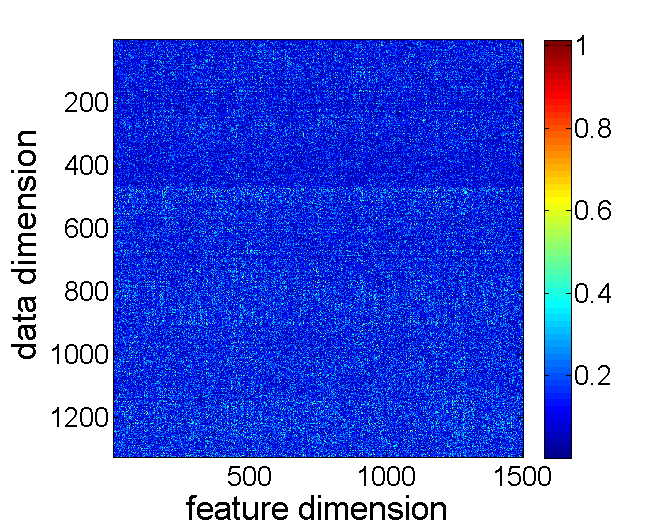
\includegraphics[width=4cm,height=3cm]{figure/Weights_summaries_in_hidden_laye_swell_exp}
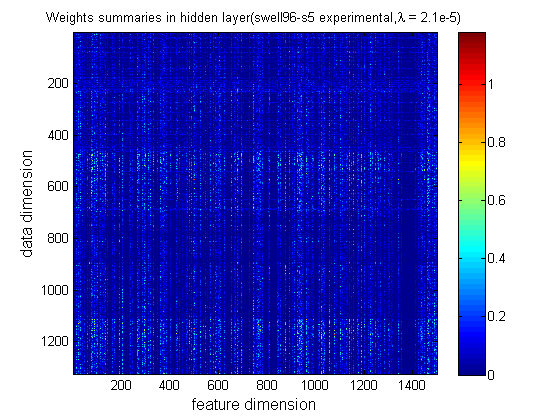
\includegraphics[width=4cm,height=3cm]{figure/Weights_summaries_in_hidden_layer_swell_exp_lambda_2_dot_1e_neg_5}
%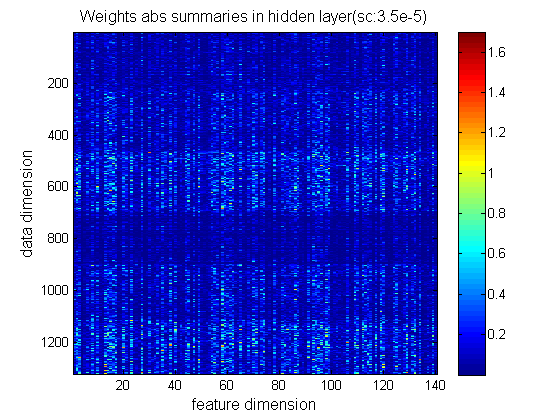
\includegraphics[width=4cm,height=3cm]{figure/Weights_abs_summaries_in_hidden_layer_sc3dot5e_nag_5_swell_140}
%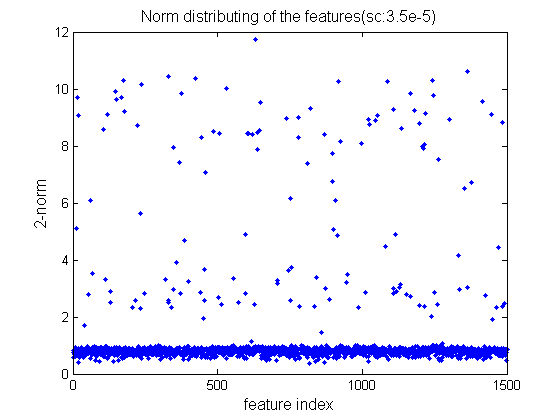
\includegraphics[width=4cm,height=3cm]{figure/Norm_distributing_of_the_features_sc3dot5e_nag_5_swell}
\caption{Weights summaries in hidden layer (left: no constraint, right: with constraint). Sparse constraint
training makes the weight coefficient show the group structure, either all zero, or basic is not zero.}
\end{figure}

Experimental data is got from SWell96Ex Event S5 vertical line array (VLA) . The array recorded a total of 75 min of data. In order to facilitate processing, 0\--50min data is took as a training set.

Consistent with the simulation part, the trajectory was divided into 300 grids, 25m each. The snapshot was set as 1-second 3000 sample-covariance matrix (SCM) would be got, the sample-covariance matrix was averaged at every two snapshots.
At the time of training, 9/10(2700)of samples were took as training set and another 1/10(300) as test set.

\subsection{The effect of sparse constraint training}
Sparsely-coded network efficiently prevents the model from over-learning, as no over-fitting occurs.
Besides, the regularization degree on model affects the model accuracy and average activation density of FNN's hidden layer. As the coefficient grows, the model accuracy on training set and test set also drops, but are slower on test set. When the coefficient is too big, the model accuracy on training set becomes much lower than test set, which indicates under-fitting.
A good constraint ratio $\lambda$ is chosen by testing in this paper.
%The model error is defined as the dissimilarity between true probability distribution and estimated probability distribution, thus the Kullback-Leibler(KL) divergence.
%In Fig.2, we use the cross entropy equivalently.

On the other hand, the regularization on neuron-level significantly reduces the average activation density.
The order of magnitude drops from $10^{3}$ to $10$, and keep it stable. This is good for us to train a sparsely-coded neural network.

Compared to the case of training without sparse constraints, sparsely-coded neural network makes the weight coefficient in the hidden layer show group structure, the element of weight vector is either all zero, or basic is not zero.
In our model, we choose $\lambda=2.1 \times 10^{-5} $, the number of feature vectors in hidden layer reduces from 1500 to 740, as shown in Fig.1. It can be seen that the relative size of learned weights is related to the frequency, and even at the same frequency, the weight corresponding
to real and imaginary parts is also different, as we can see bright and dark strips can be seen distributed along the data dimension in Fig.1. ( When we plot the weights summaries, the data dimension is arranged according to the frequency relationship from 109Hz to 385Hz.)

\begin{figure}
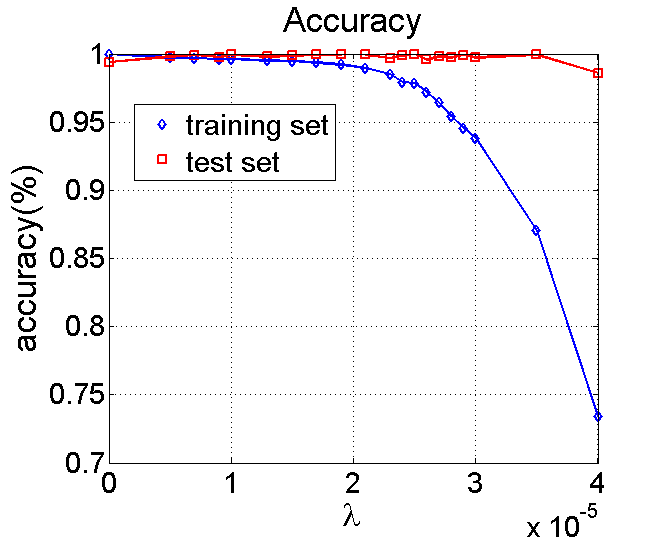
\includegraphics[width=4cm,height=3cm]{figure/Accuracy_on_SWellEx_S5_for_different_lambda}
%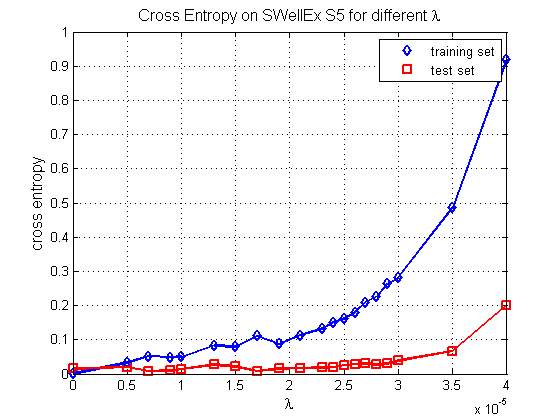
\includegraphics[width=4cm,height=3cm]{figure/Cross_Entropy_on_SWellEx_S5_for_different_lambda}
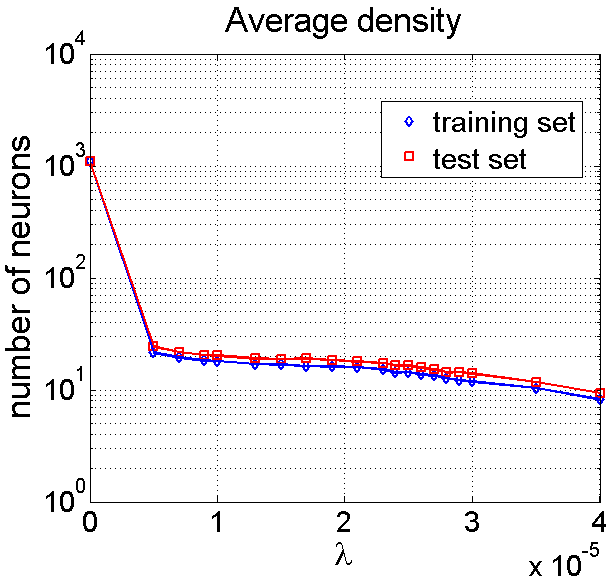
\includegraphics[width=4cm,height=3cm]{figure/Hidden_Average_Density_on_SWellEx_S5_for_different_lambda}
\caption{Model accuracy and Average-activation-density for different $\lambda $.  Regularization on neuron-level
significantly reduces the average activation density without much loss in model accuracy.}
\end{figure}


%\begin{figure}
%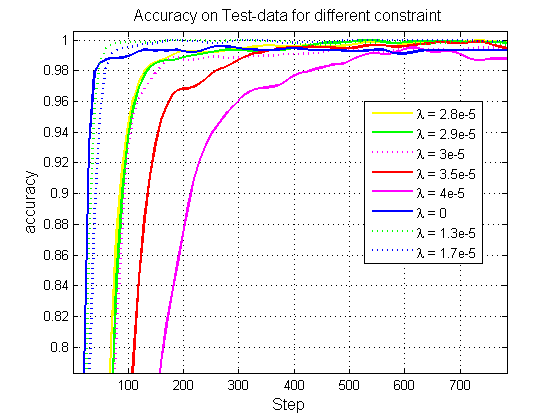
\includegraphics[width=4cm,height=3cm]{figure/Accuracy_on_Test_data_for_different_constraint_exp}
%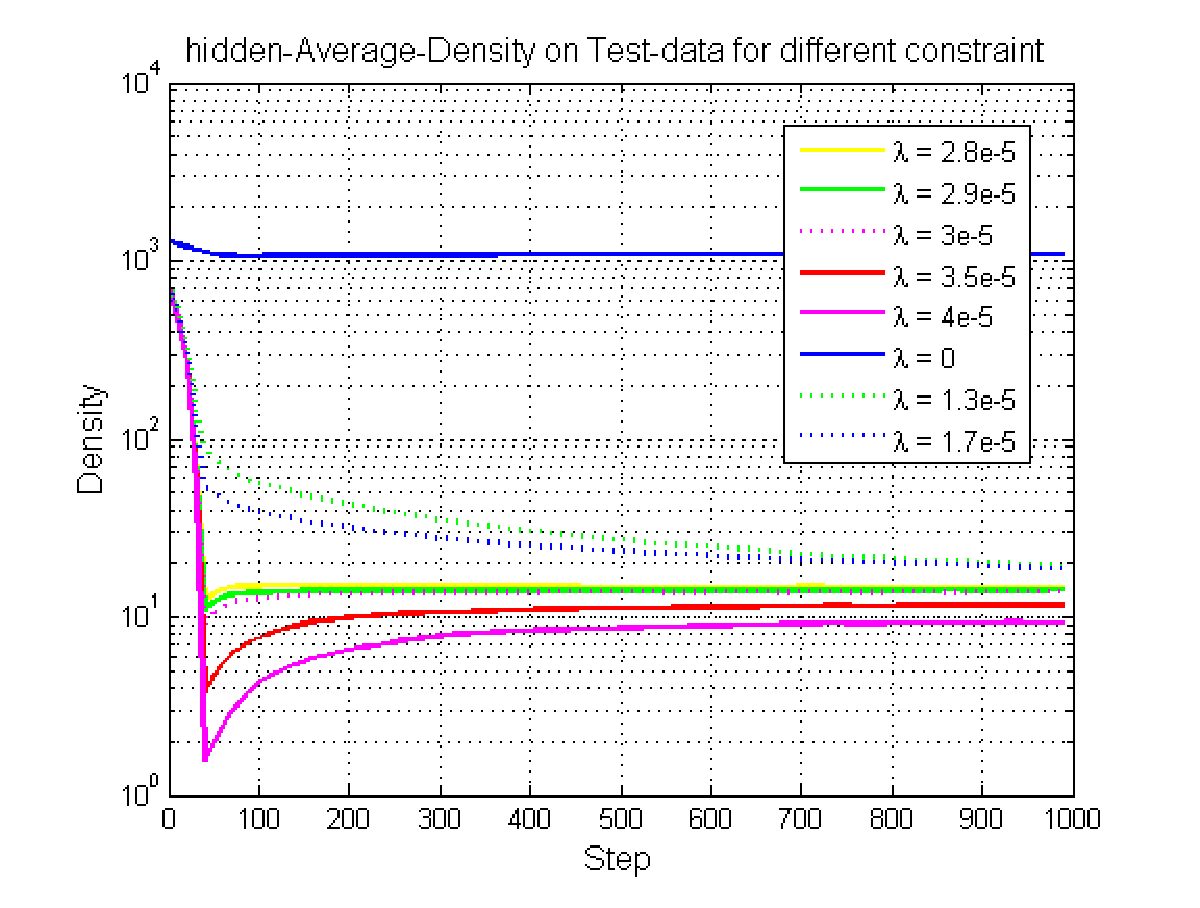
\includegraphics[width=4cm,height=3cm]{figure/hidden-Average-Density-on-Test-data-for-different-constraint_exp}
%\caption{Accuracy and Average-Density on test data for different-constraint.}
%\end{figure}

%\begin{figure}
%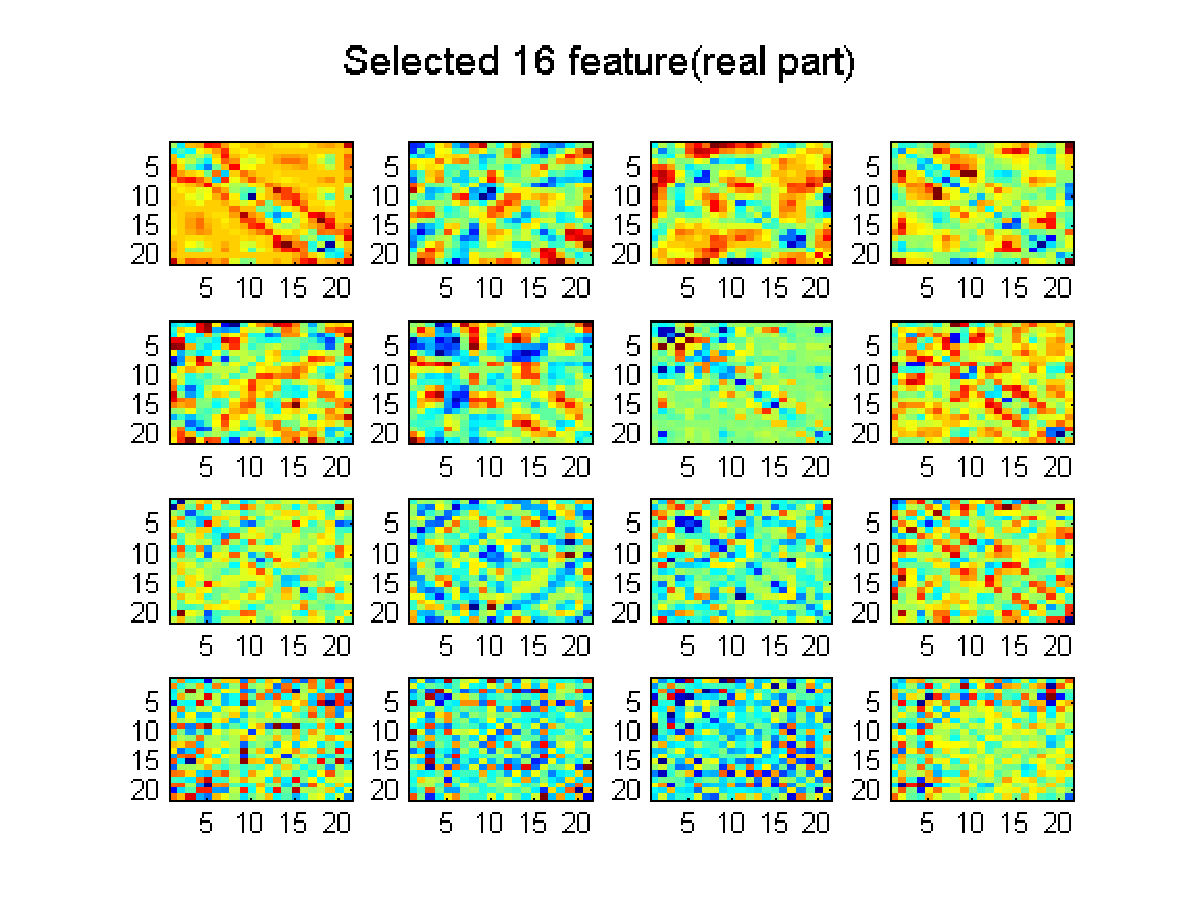
\includegraphics[width=4cm,height=3cm]{figure/selected_16_features_real_part}
%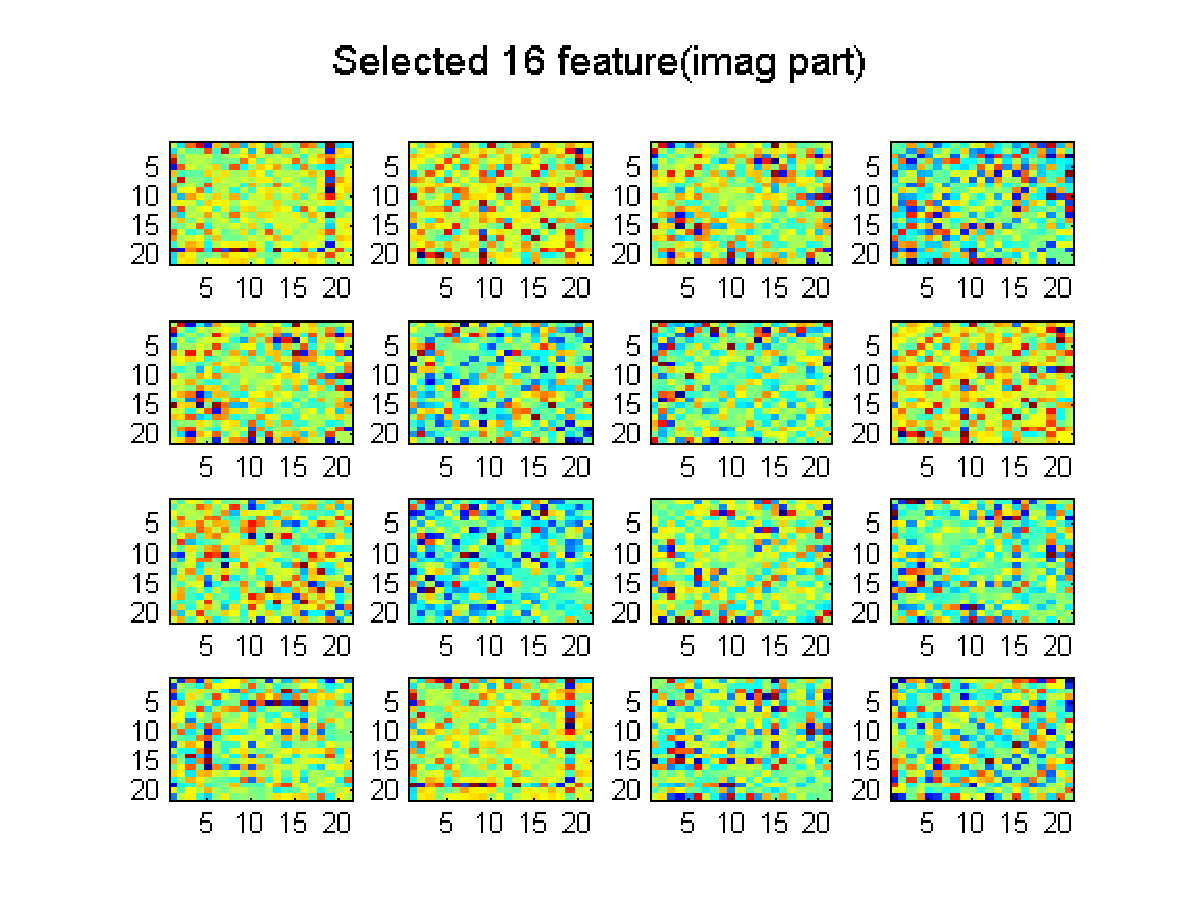
\includegraphics[width=4cm,height=3cm]{figure/selected_16_features_imag_part}
%\caption{Selected 16 features learned by neural network.}
%\end{figure}

\begin{figure}
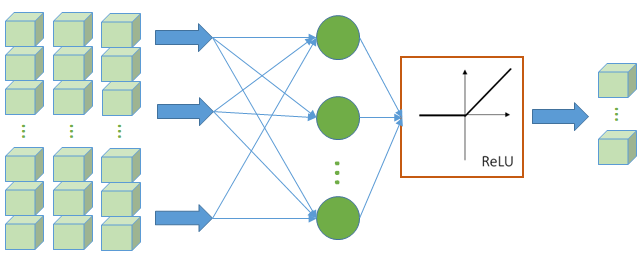
\includegraphics[width=8cm]{figure/sparse_represention_model}
\caption{The learned sparse representation model. The learned feature space spans data(scm) space likelihood that few basis functions $\phi$ explain a given data.}
\end{figure}

Apart from being beneficial to feature selection, sparse constraint also reduces the activation rate of neurons in the hidden layer. In our model, i.e. the coefficient is 2.1e-5, the average activation neuron number is just 16, which is greatly reduced, the activation rate is only 1.1{\%}.
This means, the input 1323-elements SCM  data space can be spanned by the 740 feature vectors, and averagely, each data sample can be represented by only 16 feature. To sum up, by using regularization strategy on neural networks, a sparse and low rank model is builded, where sparse means the transferred representation is sparse and low rank means the rank of learned weight matrix is low. The learned sparse coding model is illustrated in Fig.3.
A sparse vector can be formed by filtering the data measured in sensor nodes through the pre-trained sparsely-coded neuron networks.
This maybe useful for designing a decentralized source localization algorithm.%Decisions, such as target location can be made by further processing.

\subsection{Comparison with conventional matched-field processing method}
As a comparison, Bartlett processor is used here to positioning the ship source, as Niu did in his work. There are two main kinds of replica-field used in Bartlett processor, one is simulated by kraken (noted as bartlett 2), another is measurement data (noted as bartlett 1), same as the training data used in FNN.
% Please add the following required packages to your document preamble:
% \usepackage{booktabs}
\begin{table}[]
\caption{Localization accuracy of FNN and MFP on SWell96Ex-S5 data}
\label{my-label}
\begin{tabular}{@{}lllll@{}}
\toprule
Methods       & FNN    & MCE    & Bartlett 1 & Bartlett 2 \\ \midrule
109Hz         & 89.3\% & 72.3\% & 37.7\%     & 3.7\%      \\
232Hz         & 97\%   & 91\%   & 17.7\%     & 4.3\%      \\
385Hz         & 99.7\% & 97.7\% & 14\%       & 0.67\%     \\
109,232,385Hz & 99\%   & 99.7\% & 40.7\%     & 7.7\%      \\ \bottomrule
\end{tabular}
\end{table}

% Please add the following required packages to your document preamble:
% \usepackage{booktabs}
\begin{table}[]
\caption{Absolute mean error of FNN and MFP on SWell96Ex-S5 data(m)}
\label{my-label}
\begin{tabular}{@{}lllll@{}}
\toprule
Methods       & FNN  & MCE   & Bartlett 1 & Bartlett 2 \\ \midrule
109Hz         & 28.1 & 290.3 & 852.8      & 1219.5     \\
232Hz         & 7.4  & 2.5   & 832.3      & 832.3      \\
385Hz         & 0.08 & 0.58  & 1266.7     & 1756.3     \\
109,232,385Hz & 0.25 & 0.083 & 477.2      & 722.9      \\ \bottomrule
\end{tabular}
\end{table}

The accuracy and absolute mean error of different methods under different frequency are summed in table 1 and table 2. As we can see, whether in single frequency or in multi-frequency, the accuracy of FNN is always better than Bartlett, and not worse than direct data match(noted as MCE), this is more obvious when it comes to the comparison of absolute mean error.
The learned sparsely-coded neuron network works better than Bartlett processor in positioning problem.

\subsection{The influences of SSP mismatch on FNN classifier}
In the MFP method, the model accuracy is heavily affected by the mismatch problem\cite{tolstoy1989sensitivity,feuillade1989environmental,del1988effects}. Fig.5 gives the FNN positioning results by simulations in different degrees change of sound speed profiles. Here, snapshot is 10 and SNR is 5dB.
Comparing to optimized-ssp, the i905-ssp has only a very small change, within 0.5m/s at the same depth. The change in i906-ssp is much significant, which can be seen from the shape in Fig.4.
\begin{figure}
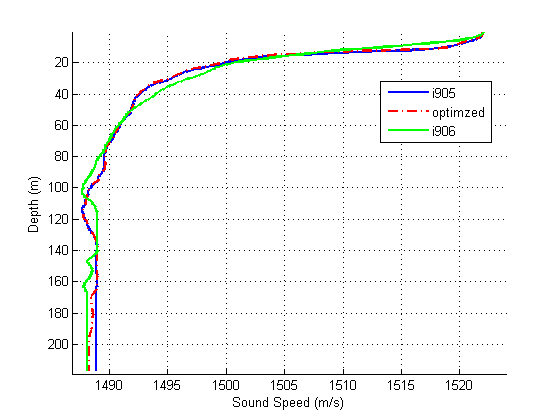
\includegraphics[width=6cm,height=5cm]{figure/ssp3}
\caption{Plots of sound speed profiles.}
\end{figure}

\begin{figure}
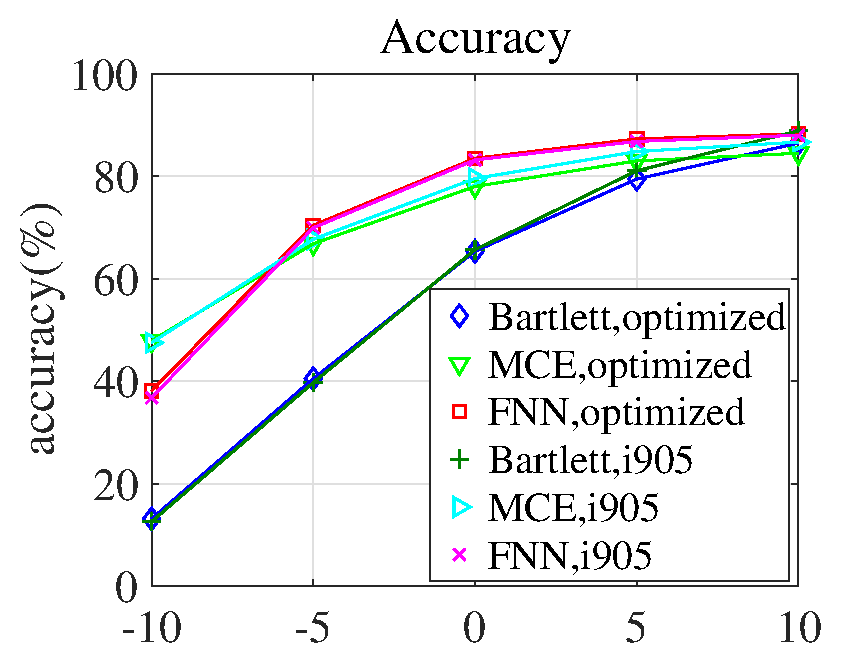
\includegraphics[width=4cm,height=3cm]{figure/Accuracy_to_SNR_FNN_vs_Bartlett_MCE}
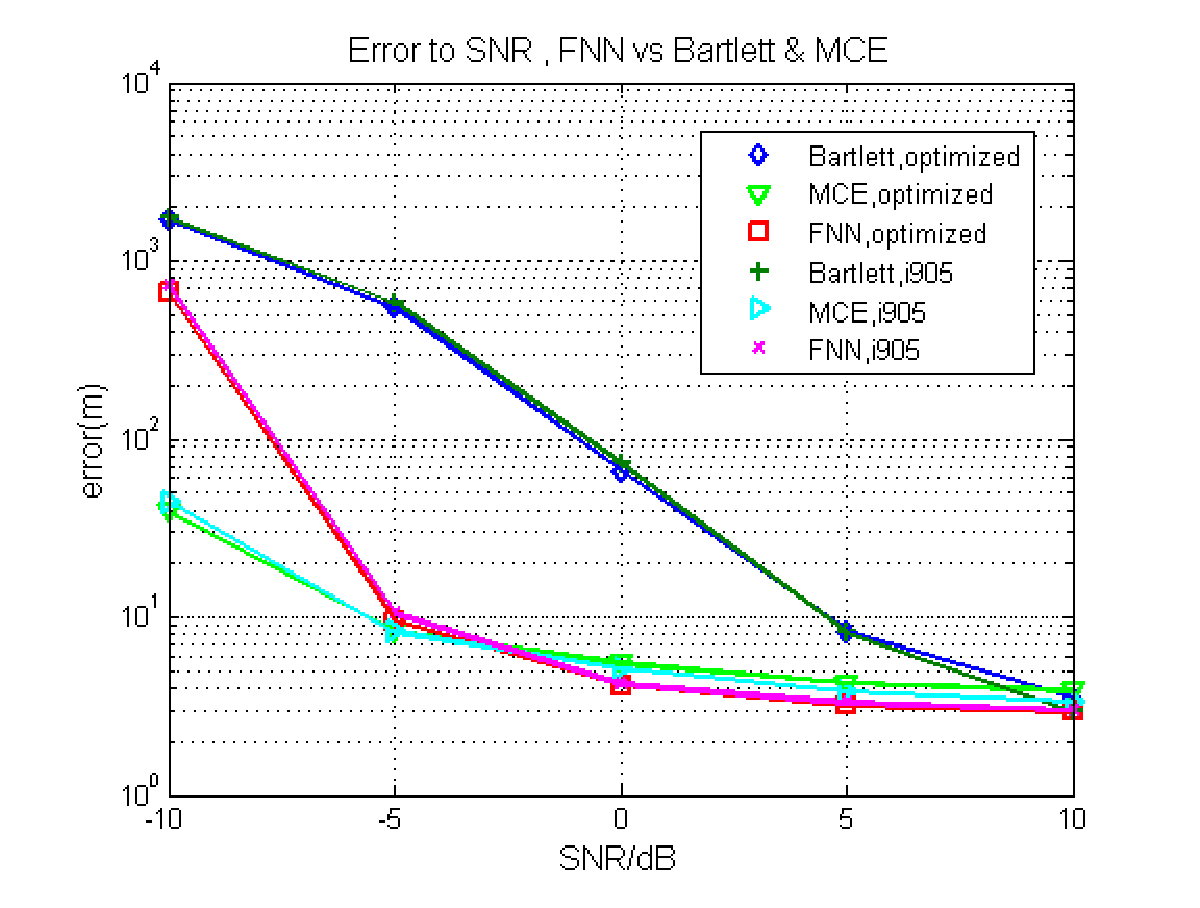
\includegraphics[width=4cm,height=3cm]{figure/Error_to_SNR_FNN_vs_Bartlett_MCE}
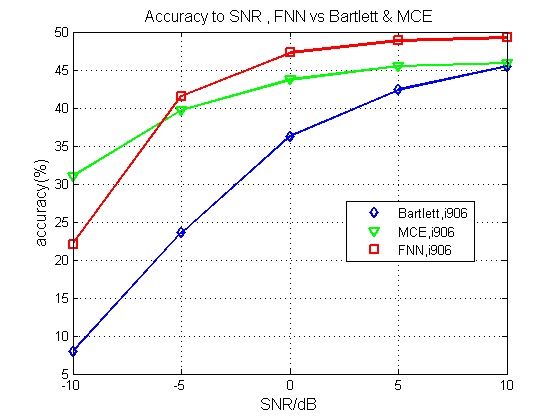
\includegraphics[width=4cm,height=3cm]{figure/Accuracy_to_SNR_FNN_vs_Bartlett_MCE_i906}
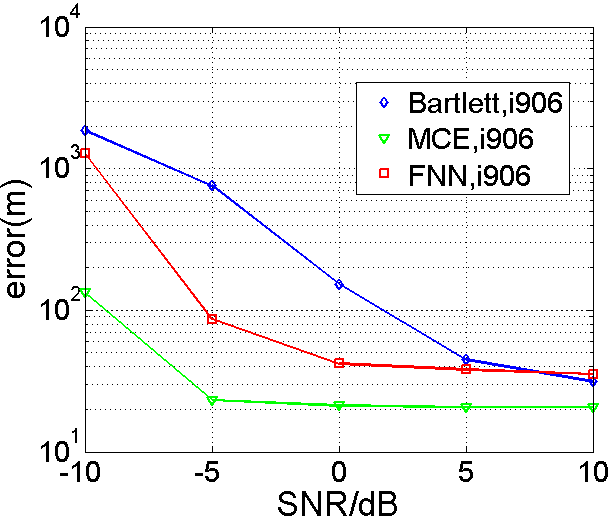
\includegraphics[width=4cm,height=3cm]{figure/Error_to_SNR_FNN_vs_Bartlett_MCE_i906}
\caption{FNN positioning performance curve on simulation data(frequency:109,232,385Hz).
 FNN is also sensitive to SSP mismatch, but still performs better than MFP.
}
\end{figure}

The performance curves for FNN, Bartlett, MCE are plotted by 1000 times Monte Carlo simulation. When the change in SSP is relatively small(the up two sub figures), FNN positioning best, MCE second and Bartlett worst.
When the shape of SSP change(the down two figures), the accuracy order unchanged, but the absolute error of FNN becomes bigger than MCE. FNN is also but less sensitive to SSP mismatch than Bartlett.

\begin{figure}
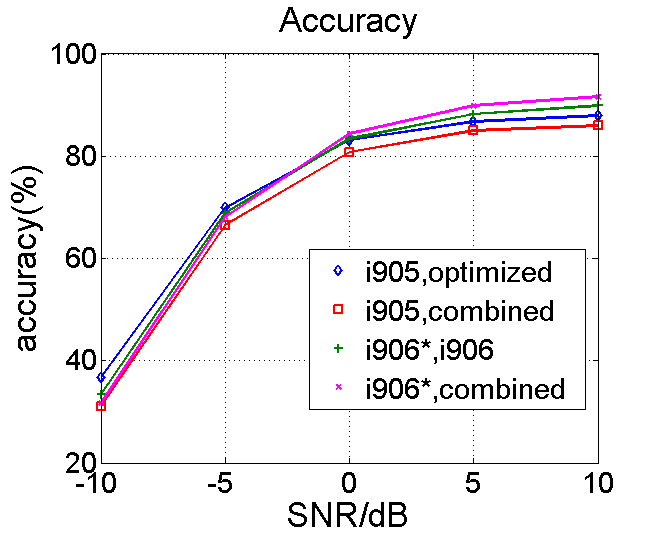
\includegraphics[width=4cm,height=3cm]{figure/Accuracy_to_SNR_Combined_vs_Single}
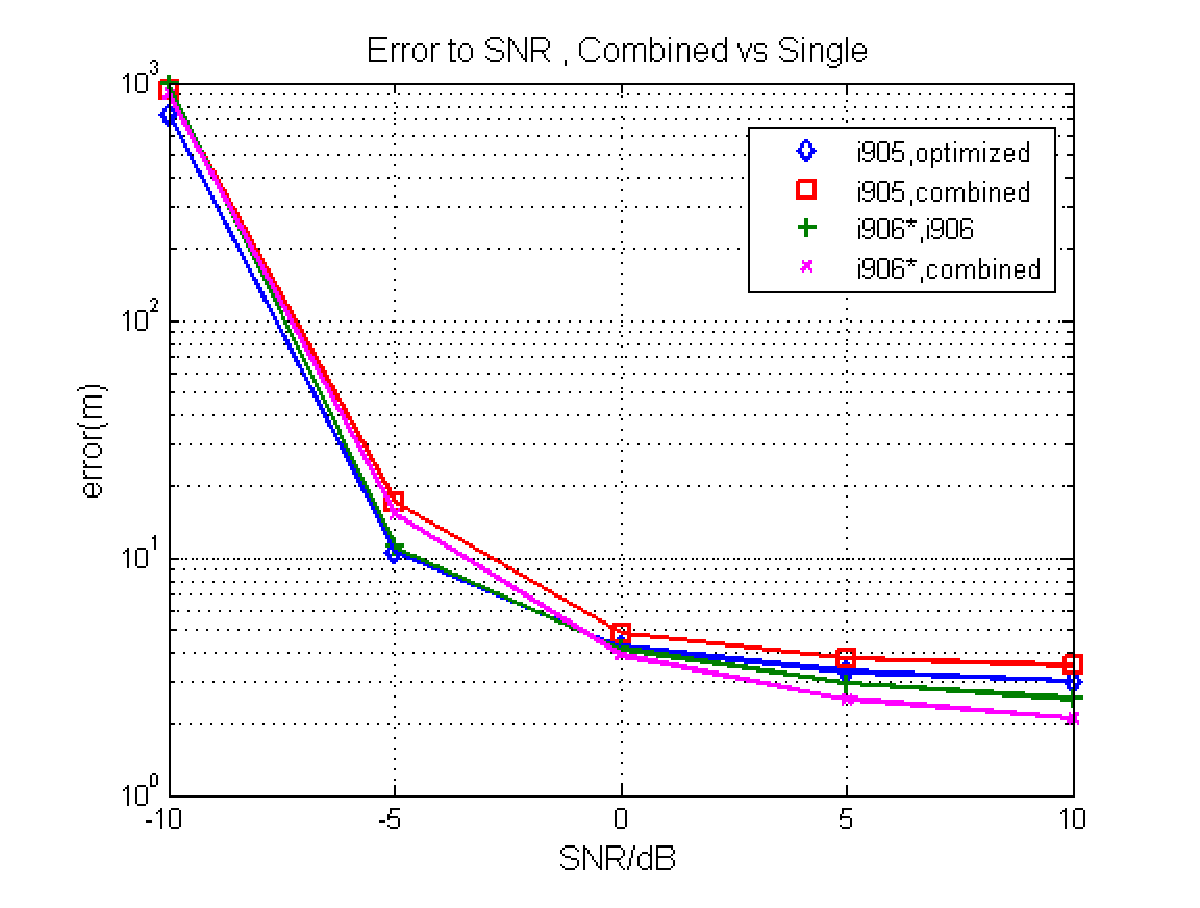
\includegraphics[width=4cm,height=3cm]{figure/Error_to_SNR_Combined_vs_Single}
\caption{FNN positioning performance curve on simulation data. FNN model robustness can be by significantly improved by data-model mixed training}
\end{figure}

\subsection{%Co-training using data collected from different ssp
Increase model robustness by data-model mixed training}
The simulation results show that training the model using data collected from different SSP can significantly improve the robustness of the classifier, which means FNN can learn weights over a set of changing SSP.

%\begin{figure}
%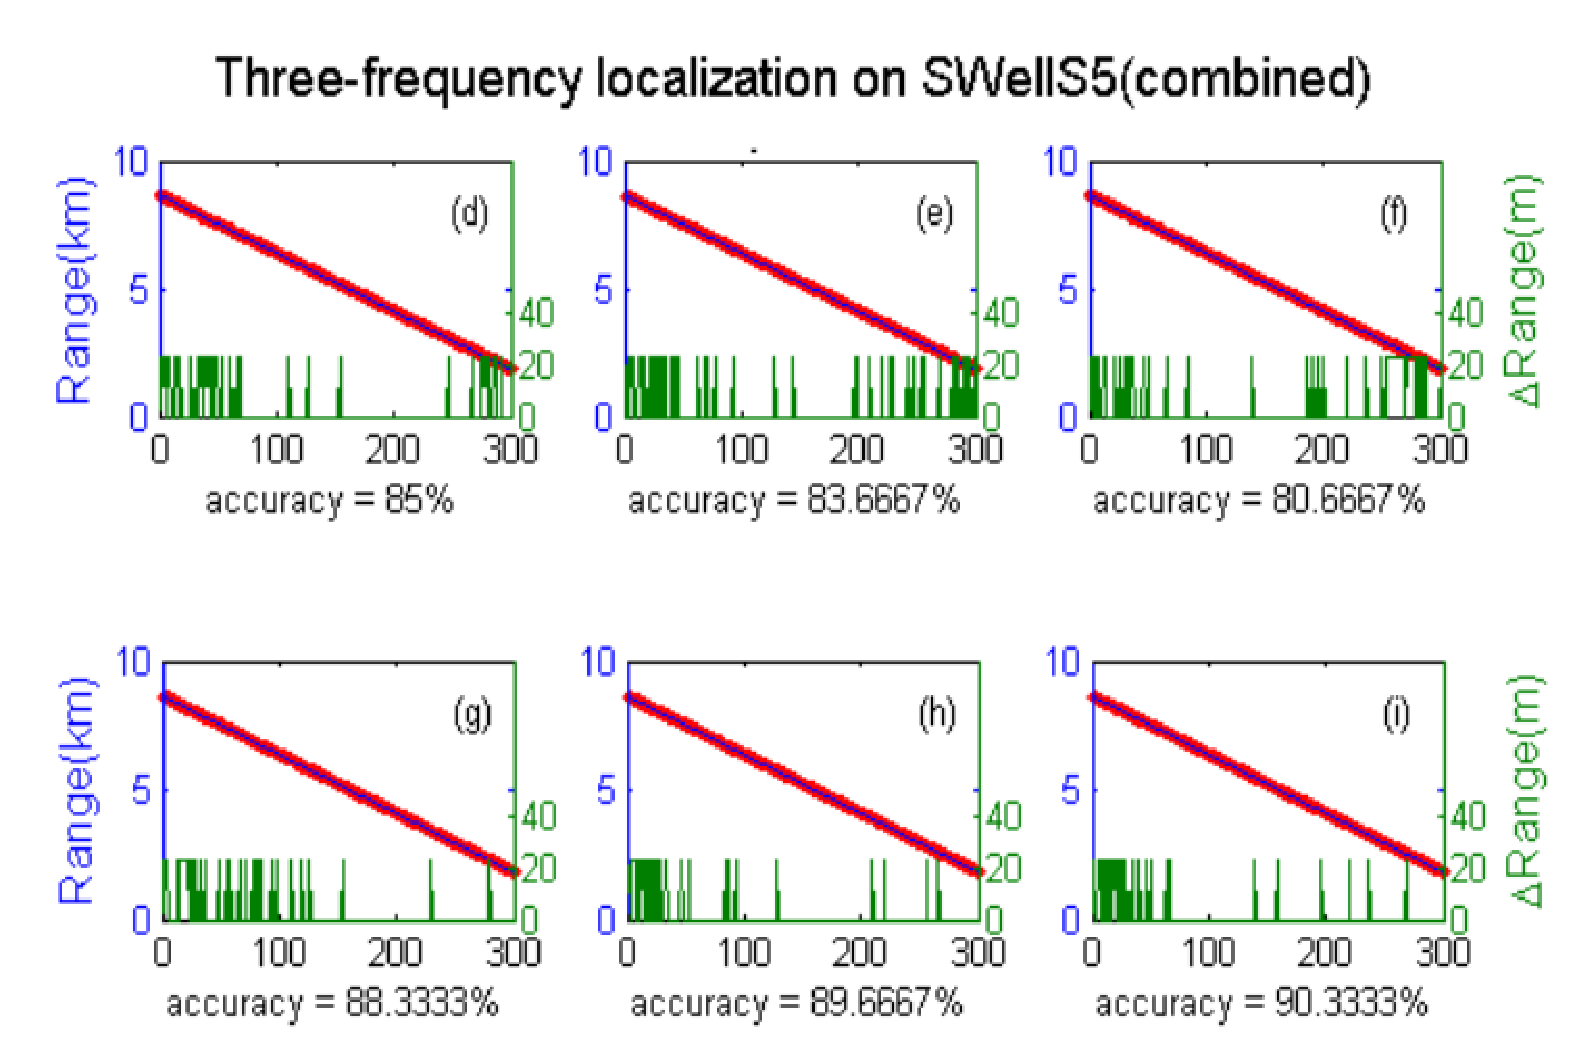
\includegraphics[width=4cm,height=3cm]{figure/combinevssingle_lef}
%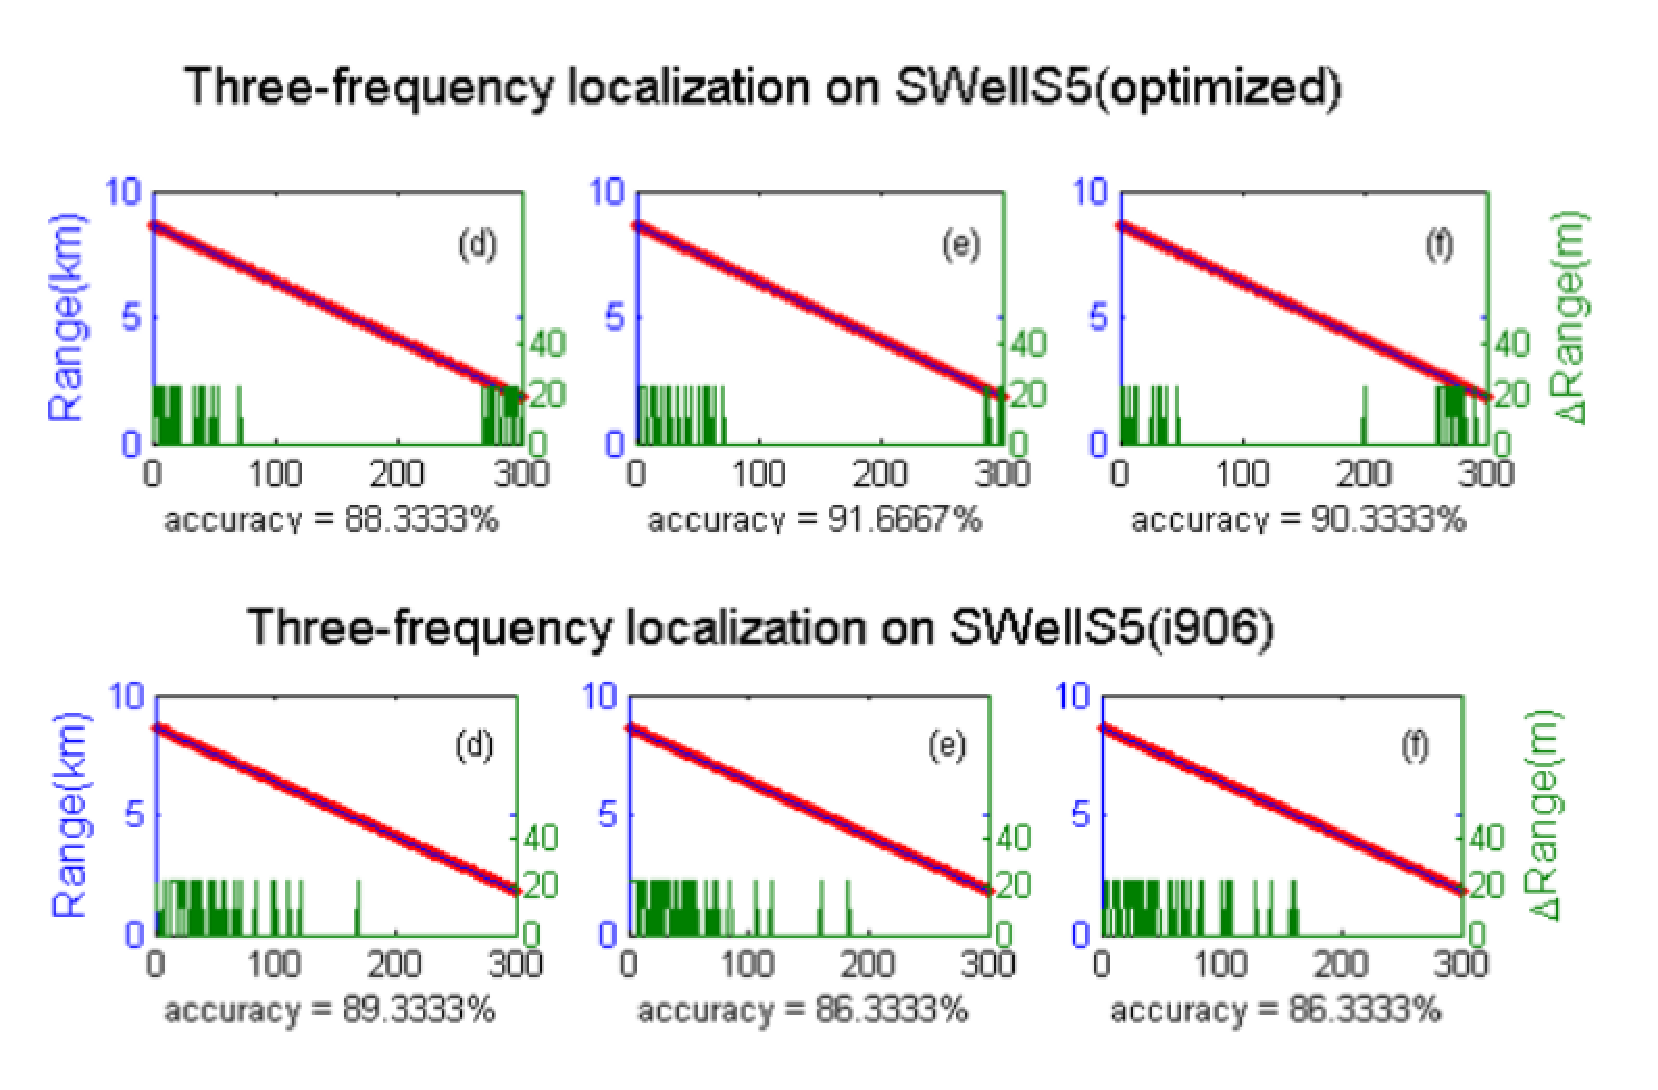
\includegraphics[width=4cm,height=3cm]{figure/combinevssingle_right}
%\caption{Comparison of mixed data training and single data training .}
%\end{figure}

As discussed in section 3.4, the FNN is also sensitive to SSP mismatch, but still performs better than Bartlett. When the environment SSP has a big change in the shape(such as from ssp-optimized to i906), the performance of the estimator drops about 40\% in accuracy. In this section, by adding data collected from i906-ssp, the positioning ability of FNN on i906{*}(which is little changed from i906,for the sake of testing) is as better as before. Although the accuracy for i905 has a little glissade compared with single data training case, the performance for i906 improved. In general, the trained FNN classifier works well on both two different shape ssp. Note that, the legend 'i905,combined' means the model is trained by mixed data collected from ssp i906 and ssp optimized, then the model is tested on ssp i905, rest legends are similar.

\section{Summary}
%In a recent article\cite{niu2017source}, Niu considers the problem of sound source location in marine waveguides as a classification problem under the framework of machine learning,and verified the ideal on the Noise09 experimental data.
%Due to the requirement for energy and computations, it is essential to develop methods to effectively exact specific task-relevant information from measures.
%It is attractive to see that neural networks model trained with sparse constraint learns a set of features with specific structures and can help construct a sparsely-coded neural network, which reduces the number of features needed to explain a given measured data. Comparing with Bartlett matched-field processing method, the neural network model performs better in mismatch cases, and it's tolerance can be obviously increased by data-model mixed training. It deserves more effort to apply more machine learning models on ocean acoustic source localization.
% It is attractive to see that the sparsely-code neural networks model predicts accurately on source localization,
% as well as the dense neural networks do, but needs fewer basis functions to span the data space.
% Combined with data-model mixed training, the model tolerance can be obviously increased,
% and performs better in sound speed profile mismatch case than Bartlett matched-field processing method.
% Machine learning methods have potential advantages in unstable underwater source localization.
% This paper primarily focus on the fine-tune for feed-forward neural networks.
% It deserves more efforts to apply complicated machine learning methods on ocean
% acoustic source localization.
It is attractive to see that the sparsely-code neural network efficiently prevents the model from over-learning and predicts accurately on source localization.
Combined with data-model mixed training, the model tolerance is obviously increased, and performs well in sound speed profile mismatch case, whether
the degree of error in knowledge is slight or large.
This ability is far superior to the Bartlett matched-field processing method.
It can be said that sparsely-coded neural network trained with mixed data-model has more potential advantages in unstable underwater
source localization.

Comparing with dense neural networks, the sparsely-code neural network needs fewer basis functions to span the data space and can make the learned weight coefficient show group structure, which is beneficial to the feature selection.
These mean the learned sparsely-code neural network model can be used not only to predict source localization, but also to describe acoustic pressure field data. This paper mainly utilizes the model to predict source localization, the descriptive ability of model need to be further exploited.
Besides, the discussion on data-model mixed training method is preliminary and just two degrees of sound-speed profiles mismatch are used to
examine the method in this paper. How will the method perform on more degrees of mismatch cases? Whether a strong enough model could be trained to suit for all sound-speed profile mismatch cases? These two questions are valuable research issues and await to be studied.
For the aspect of machine learning methods, this paper simply use a fine-tuned feed-forward neural network,
it deserves more efforts to apply more complicated machine learning methods, such as convolutional neural networks, recurrent neural networks or other deep neural networks on ocean acoustic source localization.

\begin{acks}
The work is supported by ...
\end{acks}
